\documentclass{article}
\usepackage[utf8]{inputenc}
\usepackage{hyperref}
\usepackage{graphicx}
\usepackage[final]{ml_2020}

\usepackage{amsmath}
\usepackage{amssymb}
\usepackage{subcaption}

\usepackage[backend=biber, style = numeric, sorting = ynt]{biblatex}
\usepackage{csquotes}
\addbibresource{bibliography.bib}

\title{Can you speak like a violin ?}
\author{Clémentine Berger, Gabriela Bittencourt, Henri Desvallées, Mathilde Lefebvre, Côme Peladeau}

\begin{document}
\maketitle

\begin{abstract}
    A 200-300 word abstract describing the project, problematic, method and results.
\end{abstract}

\section{Introduction}

\section{State-of-the-art}

\section{Method}
\subsection{Build a simple VAE}

We implemented a simple VAE following \cite{Kingma2013autoecondingVariationalBayes} trained on the MNIST dataset.

The VAE's encoder has the following structure : two 2D convolutions and one linear layer, each followed by a REctified Linear Unit (ReLU) activation function, followed by :
\begin{itemize}
    \item One linear layer to compute the distribution's mean
    \item One linear layer followed by a softplus activation to compute the ditriution's variance
\end{itemize}

The decoder then has the following structure : 
one linear layer followed by two 2D transposed convolution layers, with two ReLU activations and one Sigmoid activations functions.

The loss is then the sum between the reconstruction error and the Kullback-Liebler Divergence ($D_{KL}$), with a $\beta$ factor \cite{Higgins2017betaVAELB}, the reconstruction error being the binary cross entropy between the input image and the decoded output image \ref{eq:betaVAELoss}.

\begin{equation}\label{eq:betaVAELoss}
    \mathcal{L} = \mathbb{E}_{q_\phi(z|x)}[\log [p_\theta(x|z)] - \beta D_{KL}(q_\phi(z|x)||p(z))
\end{equation}



\subsection{Build a simple DCGAN}

As well as creating a simple VAE, we implement a simple convolutional \textit{Generative Adversarial Network} (GAN) following the DCGAN model that we are first going to train on the MNIST dataset.

The following structure is implemented. The discriminator is composed of two 2D convolutional layers and two linear layers. On the first three layers, we compute a batch normalization and a Leaky ReLU activation. The generator is build symmetrically with three transpose 2D convolutional layers followed by batch normalization and a ReLU activation, and finally a last convolutional layer with a Tanh activation. 

Firstly we use a Binary Cross Entropy (BCE) loss, as used in the original paper, and an Adam optimizer on both the discriminator and the generator. 

In order to avoid instabilities due to vanishing gradient or mode collapse issues, in a second time we replace the BCE loss by a Least Square GAN (LSGAN) loss. 

\begin{figure}
    \centering
    \begin{subfigure}[b]{\textwidth}
        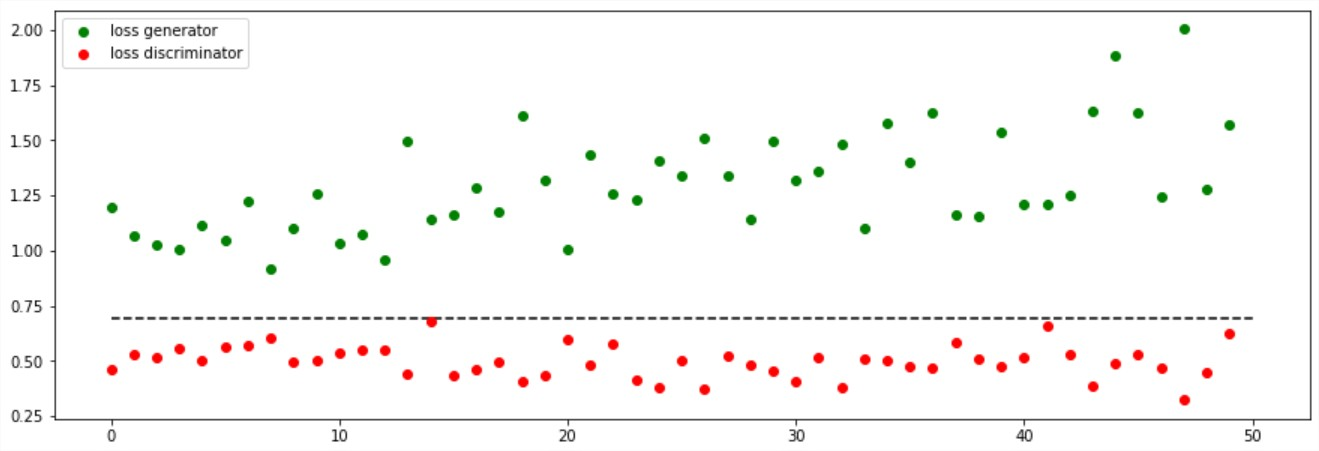
\includegraphics[width=\linewidth]{simple_dcgan/loss_BCE.jpg}
        \caption{BCE loss}
    \end{subfigure}
    \begin{subfigure}[b]{\textwidth}
        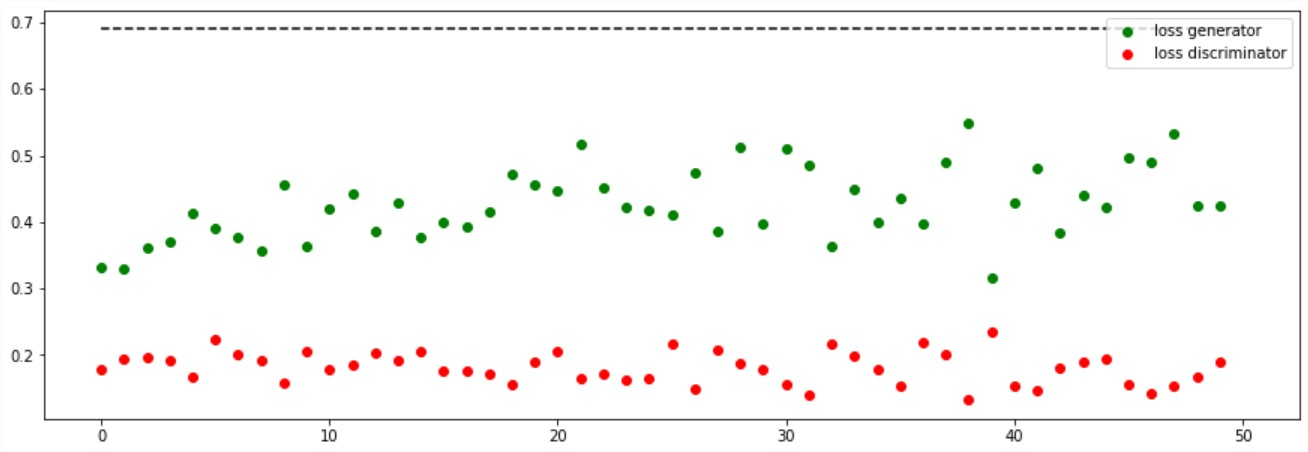
\includegraphics[width=\linewidth]{simple_dcgan/loss_MSE.jpg}
        \caption{MSE loss (Least Square)}
    \end{subfigure}
    \caption{}
    \label{fig:my_label}
\end{figure}   %à modifier dans la structure finale


\section{Experiments}

\section{Results}

\section{Conclusion}

\printbibliography
\end{document}